
% File eamt15.tex, an adaptation of eamt14.tex (which was a copy of
% eamt12.tex)
%
% Contact: eamt2015@dlsi.ua.es

%%% To ease future customizations, various replaceables have been paramaterized
%%% as listed in the newcommands section

\documentclass[11pt]{article}
\usepackage{eamt15}
%\usepackage{times}
\usepackage{latexsym}
\setlength\titlebox{6.5cm}    % Expanding the titlebox
%%% YOUR PACKAGES BELOW THIS LINE %%%
\usepackage{url}

\usepackage{multirow}


\usepackage{polyglossia}
\usepackage{todonotes}
\setdefaultlanguage[variant=australian]{english}
\usepackage{latexsym}
%\usepackage[small,bf]{caption}
\usepackage[bf]{caption}
\usepackage{xltxtra}
\usepackage{times}
\usepackage{fontspec}
\usepackage{footnote}
\usepackage{natbib}
\defaultfontfeatures{Scale=MatchLowercase,Mapping=tex-text}
\usepackage{listings}
\usepackage{microtype}
\newcommand{\anonymize}[1]{\phantom{#1}}
%\newcommand{\anonymize}[1]{#1}


\newfontfeature{IPA}{+mgrk}
%\setromanfont[IPA]{FreeSerif}
%\setromanfont[Scale=0.9]{Times New Roman}
\setromanfont{Times New Roman}
\newfontfamily\qipa[IPA,Scale=MatchLowercase]{FreeSerif}
\newfontfamily\qipb[IPA,Scale=MatchLowercase]{Junicode}
\setmonofont[Scale=0.7]{DejaVu Sans Mono}
\newfontfamily\smallertt[Scale=0.55]{DejaVu Sans Mono}
\newfontfamily\smallerrm[Scale=0.85]{Times New Roman}

%\fontspec[FakeBold=2.5]{Times New Roman}
%\DeclareFontShape{EU1}{TimesNewRoman(0)}{m}{sc}{<->ssub * TimesNewRoman(1)/m/sc}{}



\newcommand{\confname}{EAMT 2015}
\newcommand{\website}{http://www.eamt2015.org/}
\newcommand{\contactname}{the conference chairs (Felipe
  S\'anchez-Mart\'inez, Gema Ram\'irez-S\'anchez and Fred Hollowood)}
\newcommand{\contactemail}{eamt2015@dlsi.ua.es}
\newcommand{\conffilename}{eamt15}
\newcommand{\downloadsite}{http://www.eamt2015.org/}
\newcommand{\paperlength}{$8$ (eight)}
\newcommand{\shortpaperlength}{$4$ (four)}

\newcommand{\com}[1]{\marginpar{\scriptsize #1}} 
    \setcounter{secnumdepth}{4}
\title{A free/open-source machine translation system for English to Kazakh}

\author{\anonymize{Aida Sundetova}\\
  \anonymize{Kazakh National University, } \\
  \anonymize{050040 Almaty, Kazakhstan} \\
  \anonymize{{\tt sun27aida@gmail.com}}\\
  \And
  \anonymize{\textbf{Francis M. Tyers}}\\
  \anonymize{HSL-fakultehta}\\ 
  \anonymize{UiT Norgga \'{a}rktala\v{s} universitehta} \\
  \anonymize{N-9017 Romsa, Norway} \\
  \anonymize{{\tt francis.tyers@uit.no}}
  \And
  \anonymize{Mikel L.\ Forcada}\\
  \anonymize{Dept.\ Lleng.\ i Sist.\ Informàt.} \\
  \anonymize{Universitat d'Alacant,} \\ 
  \anonymize{E-03071 Alacant, Spain} \\
  \anonymize{{\tt mlf@dlsi.ua.es}}
}


\date{}

\begin{document}
\maketitle 
\renewcommand{\baselinestretch}{0.97} % the undetectable 3% squeeze
 

\begin{abstract}
This paper presents the current state of development a shallow-transfer rule-based machine 
translation (MT) system from English to Kazakh. The main syntactic and morphological differences 
between the two languages are presented, and it is shown how the MT 
system was designed to tackle these challenges. We show an evaluation of system coverage and 
translation quality and outline and future work.
\end{abstract}

\section{Introduction}

This paper presents a shallow-transfer rule-based machine translation (MT) system from English 
(a West Germanic language) to Kazakh (a Turkic language). This is a very challenging language pair for MT.
The complex agglutinative morphology of Kazakh 
is in contrast with the simple morphology of English.
Turkic language morphology shows clear morphotactics (ordering of morphemes), but with 
complex phonological changes (morphophonology) to due to morpheme contact (vowel harmony, 
sonorisation, etc.) many of which are explicitly represented in writing.

On the other hand, there are many differences between the syntax of Turkic languages 
and English: subject–object–verb order (vs.\ subject–verb–object in English), use of 
postpositions (vs.\ prepositions in English), head-final syntax with modifiers and specifiers 
always preceding the modified/specified (vs.\ following in English), overt case marking allowing 
for a rather free ordering of arguments (vs.\ a more fixed order in English), lack of definite 
articles (extensively used in English), verbal-noun-centered structures where English uses modal 
verbs (\emph{must}, \emph{have to}, \emph{want to}) or verbal-noun or verbal-adjective-centred constructions where 
English has subordinate clauses using finite verbs with relatives or subordinating 
conjunctions (\emph{the book which I read}, \emph{the place where I saw him}, \emph{before he came}), lack of a parallel 
of the English lexical verb \emph{to have}, etc. For an account (in Russian) of 
syntactic differences between English and Kazakh, see \cite{pecherskih2012}.

We set out to build a rule-based machine translation system, because for statistical machine translation 
system we need large sentence-aligned parallel corpora, which are not freely available
for the English--Kazakh pair. An English--Kazakh statistical MT system has however recently been built by Google;\footnote{\url{http://translate.google.com}}
other work in this language pair was performed by building a small parallel corpus and using Moses \citep{assylbekov14}. Existing 
commercial systems for English to Kazakh (Sanasoft\footnote{\url{http://www.sanasoft.kz/c/ru/node/47}} 
and Trident\footnote{\url{http://www.translate.ua/us/on-line}}) both appear to be rule-based. 

This paper describes the development of a machine translation system 
for English to Kazakh using the Apertium free/open-source machine 
translation platform \citep{forcada11}. %(http://www.apertium.org). 

\section{The Apertium platform}

\begin{figure*}[htbp]
\begin{center}
 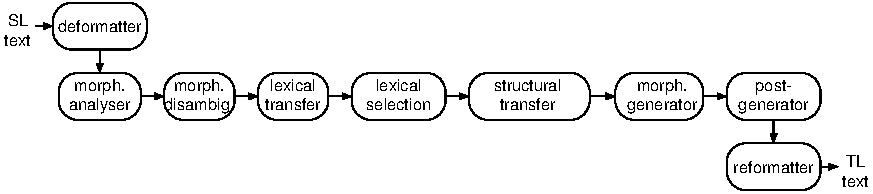
\includegraphics[width=0.8\textwidth]{architecture.pdf}
\end{center}
\caption{The pipeline architecture of the Apertium system.}
\label{figure:pipeline}
\vspace{-1em}
\end{figure*}

Apertium \citep{forcada11} is a free/open-source rule-based machine translation (MT) platform that 
has been developed since 2005, started at the Universitat d'Alacant. Apertium Was initially aimed at 
translating texts between closely related languages, then it was extended to deal with less-related 
languages. This platform has the following components: machine translation engine, developer's tools, and linguistic 
data for an increasing number of language pairs and they are licensed under the 
free/open-source GNU General Public License (GPL, versions 2 and 3). The Apertium pipeline (see figure~\ref{figure:pipeline}) has the following components:
%\todo{If space allowed, it would be nice to add a running example as in the Apertium paper}
\begin{description}\itemsep 0ex
\item[De-formatter:] Separates the text to be translated from the formatting tags.  Formatting tags are 
  encapsulated in brackets so they are treated as ``superblanks'' that are placed between words in 
  such a way that the remaining modules see them as regular blanks.  
\item[Morphological analyser:] For each surface form  (SF) the morphological analyser generates one or more 
  lexical forms (LF), which consist of: lemma (dictionary or citation form), lexical category (or part-of-speech), 
  and inflection information. 
%  In this example each source form has been analysed as one or more lexical forms: ``I'' is analysed 
%  into ``I'', where lexical category is subject pronoun (\texttt{<prn><subj>}) and first person (\texttt{<p1>}), could be 
%  masculine or feminine (\texttt{<mf>}), singular (\texttt{<sg>}); ``played'' is analysed into lexical verb (\texttt{<vblex>}) 
%  ``play'' with past simple tense (\texttt{<past>}) or it could be past participle (\texttt{<pp>}), so it has two 
%  analyses. Each analysis of word is separated by \texttt{\^{}} and \texttt{\$} symbols, and for one word each lexical 
%  forms are delimited by ``/'', and tags(<...>) show grammatical attributes of lexical form. 
\item[Part-of-speech (POS) tagger:] This module chooses one of the LFs of an ambiguous SF. 
%As can be 
%  seen from the previous example, the morphological analyser could deliver more than one LF and 
%  choosing wrong one could produce errors in translation. 
%POS tagger is based on a statistical model, which 
%  based on hidden Markov models and it has been trained on source language texts, which processes the 
%  result of the application of  on constraint-grammar rules \citep{karlsson95}, which are used to discard some 
%  analyses using rules based on context. 
%For example, consider the morphological analysis of word ``book'':
%\begin{verbatim}
%^book/book<n><sg>
%/book<vblex><inf>
%/book<vblex><pres>$
%\end{verbatim}
%  This word has 3 lexical forms, and depends on context, ont of them will be chosen by rules or tagger. 
%After  this module, all words have only one morphological analysis.
\item[Lexical transfer:] It reads each source-language LF and delivers the corresponding target-language 
  LFs. This module uses a bilingual dictionary. 
%For the English--Kazakh language pair, each lexical form of 
%  English word is translated into Kazakh as follows:
%\begin{verbatim}
%^I<prn><subj><p1><mf><sg>/мен<prn><pers><subj><p1><mf><sg>$ 
%^play<vblex><past>/ойна<v><tv><past>$
%\end{verbatim}
 Multiword units can be translated as a single LF.
\item[ Lexical selection:] It uses rules to select one of the target-language LFs, as described in \cite{tyers12a}.
\item [Structural transfer:] This module uses pattern matching to identify sequences of LFs (phrases or 
  segments), which need syntactical processing.
%to deal 
%with grammatical differences between two languages (handling of 
%  number, gender, etc.). 
It uses files with rules, which specify syntactic transformations such as word reorderings, 
  lexical changes such as changes in prepositions, and agreement between target language lexical forms. %Transfer rules can 
%  produce new sequences for the  target language, for instance, preposition-noun rule is used to build a sequence, where for 
%  noun is chosen right case, which depends on preposition.
%\begin{verbatim}
%in garden  --  ^бақша<n><sg><PXD><loc>$
% \end{verbatim} 
\item[Morphological generator:] It transforms the sequence of target-language LFs, produced by the structural transfer, 
  to a corresponding sequence of target-language SFs. 
% The morphological generator executes a finite-state transducer 

\item[Post-generator:] Performs some minor orthographical operations in the target language.\footnote{This module is not used when the target language is Kazakh.} 
\item[ Reformatter:] It places format tags back into the text so that its format is preserved.
\end{description}

\section{Linguistic data}

Apertium uses text-based (mainly XML-based) formats for linguistic
data, which include bilingual and monolingual dictionaries, structural
transfer and lexical selection rules.

\subsection{Dictionaries}

Dictionaries are used in lexical processing: monolingual dictionaries
for morphological analysis of English and generation of Kazakh and
bilingual dictionaries for English--Kazakh lexical transfer.  

Morphological dictionaries are used to define the correspondences between LFs and SFs; they contain a definition of the source-language alphabet and grammatical categories and attributes (such as noun, verb, plural, locative, etc.), a list of all lexical units, and inflection paradigms for all lexical categories; paradigms describe regularities in the correspondences
between parts of SFs and LFs.  

The English dictionary comes from existing data in Apertium, such as the English---Spanish language pair.

The Kazakh dictionary \citep{washingtonsalimzyantyers14} is turned
into a finite-state morphological transducer, using the Helsinki
Finite State Toolkit \citep{hfst/2011}. The dictionary is based on
two-level rules, and uses the \texttt{lexc} formalism for defining
lexicons through word classes and subclasses, and the \texttt{twol}
formalism for morphophonological rules such as vowel harmony,
desonorization, nasalization, etc. An example of morphophonological
rule: depending on the preceding vowels and consonants, the plural
suffix \emph{-LAr}\footnote{Uppercase Latin letters are used for
  archiphonemes (actually archigraphemes) that are realised as
  phonemes (actually graphemes) after morphophonological rules have
  been applied.} for noun could become \emph{-тар}, \emph{-тер}, \emph{-лар},
\emph{-лер}, \emph{-дар}, \emph{-лер}:
кітап+тар, мектеп+тер, etc.


%\subsubsection{Bilingual dictionary}

The English--Kazakh bilingual dictionary provides correspondences between English LFs and Kazakh LFs. Ambiguity is allowed: one of the LFs will be chosen by 
lexical-selection rules depending on context (see below). This dictionary currently contains 13,135 stems \citep{sundetova13a}.

\subsection{Rules}

\subsubsection{Disambiguation rules}

The problem of part-of-speech (PoS) ambiguity is solved using the  Constraint Grammar (CG, \cite{karlsson95}) formalism: CG rules choose one of the LFs obtained for each SF. %From English to Kazakh POS ambiguity could be only in English side, but also some choice also
%depend on Kazakh grammar.\todo{I removed an unclear sentence here}

\subsubsection{Lexical selection rules }

Lexical-selection rules choose one of the alternative target-language LFs corresponding to one source-language LF, as described by \cite{tyers12a}. Alternative translations are defined in bilingual dictionary by 
multiple entries for each source-language LF. For example, the adjective \emph{beautiful} could be translated as \emph{сұлу}, if 
the following noun is a person: \emph{beautiful girl} \(\to\) \emph{сұлу қыз}; or as \emph{әдемі} or  \emph{көркем}, if the following noun means 
place: \emph{beautiful mountains} \(\to\) \emph{әдемі таулар}.  Table~\ref{table:lexsel} shows examples of 
lexical-selection rules:

\begin{table*}
 \centering
 \begin{tabular}{|l|l|l|l|}
    \hline
    \textbf{SL word \(w\)} & \textbf{TL word} & \textbf{Context} & \textbf{Example} \\
    \hline
    \multirow{4}{*}{residence} & \multirow{2}{*}{мекен}      & \multirow{2}{*}{default} & I live in a residence. \\
                               &                             &                     & (Мен) мекенде өмір сүремін. \\
                               & \multirow{2}{*}{резиденция} & \multirow{2}{*}{\(w\)\_ of \_ president} & I see the residence of the president \\ 
                               &                             &                                     & (Мен) президенттің резиденциясын көремін \\
    \hline
    \multirow{4}{*}{boot} & \multirow{2}{*}{бәтеңке} & default & I bought boots. \\
                          &                          &     &  Мен бәтеңкелерді сатып алдым \\

                          & \multirow{2}{*}{жүксалғыш} & \(w\) \_ of \_ car &  He opened the boot of the car  \\ 
                          &           &              & Ол машинаның жүксалғышын ашты. \\
    \hline
    \multirow{4}{*}{anything} & \multirow{2}{*}{бір нәрсе} & default & I see anything  
\\ 
                              &           &    & Мен бір нәрсе көремін \\
                              & \multirow{2}{*}{еш нәрсе} & not \_[verb] & I do not do anything \\ 
                              &          &             &  Мен еш нәрсе істемеймін. \\

    \hline
 \end{tabular}
  \caption{Example lexical-selection rules}
  \label{table:lexsel}
\end{table*}

\subsubsection{Transfer rules}

For English--Kazakh transfer is performed in three stages \citep{sundetova13b}:

\begin{itemize}
\item A first round of transformations (``chunker'') detects source language (SL) LF patterns and generates the 
  corresponding sequences of target language (TL) LFs grouped in chunks representing simple constituents such as noun phrases, prepositional phrases, etc. 
\item The second round (``interchunk'') reads patterns of chunks and produces a new sequence of chunks. This is the 
  module where one can attempt to perform some longer-range reordering operations, interchunk agreement, case selection, etc. 
\item The third round (``postchunk'') transfers chunk-level tags to the lexical forms they contain and whose lexical-form-level 
  tags are linked (through a referencing systems) to chunk-level tags (for instance, case determined for a noun phrase is 
  transferred to the main noun), and removes all grouping information to generate the desired sequence of TL LFs.
\end{itemize}

The structural transfer module in Apertium processes the stream of source-language lexical form -- target-language lexical 
form pairs (SL LF–TL LF pairs) and transforms it into a  sequence of TL LFs after a series of structural transfer 
operations specified in a set of rules: reordering, elimination or insertion of TL LFs, agreement, etc. 

This section describes the current structural transfer in \texttt{apertium-eng-kaz}.  English--Kazakh 
chunker rules, interchunk rules and an additional clean-up stage will be described in detail in the following 3 sections. 

\paragraph{Chunker:}
In the first round of structural transfer, rules segment sentences into chunks, like short noun 
phrases, adjective phrases, verb phrases and adpositional phrases (that is, prepositional phrases in English and 
postpositional phrases in Kazakh).
Chunking rules, of which there are currently 168, identify 8 kinds of chunks and translate them into equivalent Kazakh chunks, leaving some adaptations to be performed in later stages of structural transfer (for instance, the 
morphological case of noun phrases). 

%Table~\ref{table:nps} describes what kind of noun phrases could appear in sentences and how it could be detected.\todo{This table does not add much. the first and second column of the table are essentially the same: it would be more interesting to give the Kazakh sequence of PoS tags, perhaps with an example}

% \begin{table*}
%   \centering
%   \begin{tabular}{|l|l|l|}
%   \hline
%   \textbf{Structure} & \textbf{Description} & \textbf{Examples} \\
%   \hline
%   \texttt{n} & Noun & house \\
%   \texttt{adj + n} & Adjective + noun & long road \\
%   \texttt{det + n} & Determiner + noun & an apple, the chance \\
%   \texttt{num + n} & Numeral + noun & five pieces \\
%   \texttt{num + adj + n} & Numeral + adjective + noun & five big pieces \\
%   \texttt{det + num + adj + n} & Determiner + numeral + adjective + noun & the five big pieces \\
%   \hline
%   \end{tabular}
%   \caption{Example of the most common structures of noun phrases}
%   \label{table:nps}
% \end{table*}

\begin{savenotes}
\begin{table*}
  \centering
  \begin{tabular}{|l|l|l|l|}
    \hline
    \textbf{Phrase type} & \textbf{Description} & \textbf{Examples} & \textbf{Kazakh chunk tags} \\
    \hline
    \multirow{5}{*}{\texttt{NP}} & \multirow{5}{*}{Noun phrase}    & noun & number, person, \\
                                 &                                 & determiner-noun & possessor, case\\
                                 &                                 & numeral-noun & \\
                                 &                                 & adjective-noun & \\
                                 &                                 & determiner-adjective-noun & \\
    \hline
    \multirow{5}{*}{\texttt{VP}} & \multirow{5}{*}{Verb phrase}    & finite-verb & number, person, \\
                                 &                                 & have-participle & tense/mood, possessive, \\
                                 &                                 & be-gerund & negation \\
                                 &                                 & must-infinitive & \\ 
                                 &                                 & want\_to-infinitive & \\ 
    \hline
    \multirow{5}{*}{\texttt{PP}} & \multirow{5}{*}{Postpositional phrase} & preposition-noun & number, person, \\
                                 &                                        & preposition-determiner-noun & possessor, case \\
                                 &                                        & preposition-numeral-noun & \\
                                 &                                        & preposition-adjective-noun & \\
                                 &                                        & preposition-determiner-adjective-noun & \\
    \hline
    \multirow{2}{*}{\texttt{GenP}} & \multirow{2}{*}{Genitive phrase}  & As with \texttt{PP} except & number, person, \\
                                   &                                   & with the preposition `of'. & possessor, case \\
    \hline
    \multirow{2}{*}{\texttt{AdjP}} & \multirow{2}{*}{Adjective phrase}  & adjective & (no tags) \\
                                   &                                    & ``more''--adjective & \\
    \hline
    \multirow{2}{*}{\texttt{SupP}} & \multirow{2}{*}{Superlative phrase} & adjective--``est'' & possessor, case \\
                                   &                                     & the--``most''--adjective & \\ 
    \hline
%    \texttt{Q\_mark} & Question mark  & & \\
%    \hline
  \end{tabular}
  \caption{Phrase types in the English--Kazakh chunker. }
  \label{table:phrases} 
\end{table*}
\end{savenotes}
As it is shown above, the most probable sequence of world classes are built phrases and 
for English-Kazakh chunker there are used next kind of phrases:


%% EXAMPLES ?

\begin{description}
\item[Noun phrases:] Consider the following example: the chunker identifies the English LF sequence for \emph{the large book}  (determiner--adjective--noun) as a noun-phrase chunk. It translates it into the Kazakh adjective--noun sequence \emph{үлкен кітап}, and assigns it four chunk-level tags: number (set to singular), person (set to 3rd), 
  possessor (to be determined, as the noun \emph{кітап} ('book') could receive a 3rd-person possesive 
  ending (\emph{кітабы}) later if the context were, for instance, \emph{the large book of animals}, \emph{аңдардың үлкен кіта\textbf{бы}}), 
  and case, to be determined later as it could be, for instance, accusative in \emph{I saw the large book}, \emph{Мен үлкен кітап\textbf{ты} көрдім}). Similar processing occurs for nominal forms of the verb: for instance, as in the NP \emph{her paying} in \emph{Her playing is good}, which is  \emph{Оның ойыны жақсы} (\emph{She}+\textsc{genitive} \emph{playing}+\textsc{poss-3rd} \emph{good}). 
\item[Prepositional phrases:] English prepositional phrases are translated into Kazakh as postpositional phrases, 
  there are three possible outcomes with different cases:
   \begin{itemize}
    \item Genitive \emph{-NIң},\footnote{In the genitive ending \emph{-{N}{I}ң}, the archiphoneme {N} may be realised as т, д, or н and the archiphoneme {I} may be realised as  і  or ы depending on the previous phonological context. } in which will case the phrase will be marked GenP:  
        [PP [P \emph{of} ] [NP \emph{the beautiful garden}] ] $\rightarrow$ [GenP [NP \emph{әдемі бақша}] [P \emph{-ның}] ] 
    \item Translating into any of the morphological cases: locative \emph{-{D}{A}}'',\footnote{\emph{D} can be \emph{д} or \emph{т}, and \emph{{A}} can be \emph{е} or \emph{а}, depending on the 
        phonological context.} ablative \emph{-{D}{A}н}, etc. --- all except the genitive \emph{-{N}{I}ң} case: 
        [PP [P \emph{from} ] [NP \emph{the five cars}] ] $\rightarrow$ [PP [NP \emph{бес көлік}] [P \emph{-тен} ] ]
    \item Using postpositional constructs based on positional nouns such as \emph{аст} (`under'), \emph{үст} (`on'), etc., which take the possessive from the main noun:  
        [PP [P \emph{under} ] [NP \emph{the garden}] ] $\rightarrow$ [PP [NP [GenP [NP \emph{бақша} ][P \emph{-ның}]] [NP \emph{аст\textbf{ын}}]] [P \emph{-да} ] ]
    \end{itemize}
\item[Verb phrases:] Translation of English verb phrases into Kazakh is not always be straightforward. For instance,
tenses expressing continued activity, such as the 
  English present continuous or past continuous (\emph{I am playing}, \emph{I was playing}), have to be detected and 
  mapped onto sets of two lexical units (\emph{Мен ойнап жатырмын}, \emph{Мен ойнап отырдым}) where the main verb is 
  found in the \emph{-п} participle form (\emph{ойна\textbf{п}}), and a suitable finite form  (\emph{жатырмын}, \emph{отырдым}) of an auxiliary 
  verb (\emph{жатыр}, \emph{отыр}) is used to express number and person agreement\footnote{Actually, Kazakh uses four auxiliary verbs: \emph{жатыр} `lie', 
      used when the activity takes a long time), отыр (`sit', used when the activity appears to be done in a sitting position), \emph{тұр} `stand', 
      when the takes a short time), and \emph{жүр} (when the activity repeats regularly). Choosing the most adequate auxiliary verb is 
      hard without a semantic analysis, which is not easily available in Apertium. Our current choice (an approximation) 
      is \emph{жатыр} `lie' for the present continuous and отыр (`sit') for the past continuous.}. Modal verbs are translated by adding adjectives, which means \emph{керек} `necessary' or \emph{жөн} `proper', 
  and a form of the copula (absent in present tense), with the subject receiving the genitive or dative case. Negative 
  verbs for present continuous and past tense are translated by adding the negative word \emph{емес} for present 
  perfect continuous (\emph{He has not been playing} \(\to\) \emph{Ол ойнап отырған емес}) and  \emph{жоқ} for past tense and 
  present continuous.
\item[Adjectival phrases:] In Kazakh noun phrases, adjectives come before nouns and do not show any agreement 
  with nouns.  Adjectives can also appear in separate adjective phrases. Here are some examples:
\begin{itemize}
\item The adjective alone, marked AdjP: [AdjP \emph{big} ] $\rightarrow$ [AdjP \emph{үлкен}] 
\item Comparative adjective phrases  (English \emph{more} + adjective, or adjective-[\emph{e}]\emph{r}); the Kazakh translation 
   chooses the comparative suffix \emph{{I}р{A}{K}}: [AdjP  \emph{more  interesting} ]  $\rightarrow$ [AdjP \emph{қызығ\textbf{ырақ}}]
\item For superlative adjective phrases  (\emph{the most} + adjective  or adjective-[\emph{e}]\emph{st}, translation 
   is built using \emph{ең} + adjective:  [SupP  the \emph{biggest} ]  $\rightarrow$ [SupP \emph{ең үлкен}] 
   [SupP  \emph{the most important}]   $\rightarrow$ [SupP \emph{ең маңызды}].
\end{itemize}
Superlative adjective phrases have some properties of noun phrases (such as receiving possessive morphemes when 
modified by a genitive phrase: \emph{the most beautiful of people} $\rightarrow$ \emph{адамдардың ең әдемі\textbf{сі}}); they are treated as a noun phrase with an implied noun (\emph{the largest} [\emph{book}]).

\end{description}

\begin{table*}
  \centering
  \begin{small}
  \begin{tabular}{|l|l|l|l|}
    \hline
    \multicolumn{4}{|c|}{\textbf{Affirmative forms}} \\
    \hline
    \textbf{English form} & \textbf{Example} & \textbf{Morphemes} & \textbf{Translation} \\
    \hline
    \multirow{2}{*}{Present simple} & \multirow{2}{*}{\emph{I play}} & \multirow{2}{*}{\emph{ойна} + <aorist> + <pers.>} & \emph{Мен ойнаймын} \\
                                    &                         &                                            & 'I play' \\
    \hline
    \multirow{2}{*}{Present continuous} & \multirow{2}{*}{\emph{I am playing}} & \emph{ойна} + <perf. part.>  & \emph{Мен ойнап жатырмын} \\
                                    &                         &   \emph{жатыр} + <pres.> + <pers.>     & 'I playing lie' \\
    \hline
    \multirow{2}{*}{Past continuous} & \multirow{2}{*}{\emph{I was playing}} & \emph{ойна} + <perf. part.>  & \emph{Мен ойнап отырдым} \\
                                    &                         & \emph{отыр} +  <past>  + <pers.>     & 'I playing sat' \\
    \hline
    \multirow{2}{*}{Obligation} & \multirow{2}{*}{I must go} & \emph{Мен}  + <gen.>  & \emph{Менің баруым керек} \\
                                    &                         & \emph{бар} + <ger.> +  <poss.\ p1 sg.> + \emph{керек}    & 'My going necessary [is]' \\
    \hline
    \multirow{2}{*}{\emph{Should}} & \multirow{2}{*}{\emph{I should go}} & Мен  + <gen.>  & \emph{Менің барғаным жөн} \\
                                    &                         & \emph{бар} + <past.ger.> +  <poss.\ p1 sg.> + \emph{жөн} & 'My having gone proper is' \\
    \hline
    \multicolumn{4}{|c|}{\textbf{Negative forms}} \\
    \hline
    \multirow{2}{*}{Present cont.} & \multirow{2}{*}{\emph{I am not playing}} & \emph{ойна} + <perf. part.>  & \emph{Мен ойнап жатқан жоқпын} \\
                                    &                         &   \emph{жатыр} + <pres.> + <pers.>     & 'I playing lying not' \\
    \hline
    \multirow{2}{*}{Inability} & \multirow{2}{*}{\emph{I can not play}} & \emph{ойна} + <impf. part.>  & \emph{Мен ойнай алмаймын} \\
                                    &                         &   \emph{ал} + <neg.> + <aor.> + <p1>     & 'I playing cannot' \\
    \hline
    \multirow{3}{*}{Present perf. cont. } & \multirow{3}{*}{\emph{You have not been playing}} & \emph{ойна} + <perf. part.>  & \emph{Сіз ойнап отырған емессі} \\
                                    &                         & +  \emph{отыр} + <past>  & 'You playing sat not'  \\
                                    &                         & + \emph{eмес} <cop.neg> + <p2> & \\
    \hline
    
     
  \end{tabular}
  \end{small}
  \caption{Examples of verb-phrase translations}
  \label{table:vps}
\end{table*}

\paragraph{Interchunk processing:}

The second round of structural transfer is currently performed by a %proof-of-concept 
set of 140 rules, representative of following operations:
\begin{itemize}
\item Persona and number agreement between the subject noun phrase and the verb phrase.
\item Assigning case to noun phrases (which are generated without case by the chunker): for instance, 
  accusative case for objects (\emph{I bought the table} $\rightarrow$ \emph{Мен үстел\textbf{ді}  сатып алдым}), genitive case for 
  obligatory constructs (\emph{I must see} $\rightarrow$ \emph{ме\textbf{нің} көруім керек}),  dative case for the verb \emph{to 
  need} (\emph{I need a doctor} $\rightarrow$ \emph{Ма\textbf{ған} дәрігер керек}), locative case for 
  possession (\emph{I have a book} $\rightarrow$ \emph{Мен\textbf{де} кітап бар}), etc.\ 
 \item Reordering: placing of object before verb ( \emph{I}$_1$ \emph{bought}$_2$ \emph{the table}$_3$ $\rightarrow$ \emph{Мен}$_1$ \emph{үстелді}$_2$ \emph{сатып алдым}$_2$), 
  placing of prepositional phrases before the verb  (\emph{They}$_1$ \emph{played}$_2$ \emph{on top of the tree}$_3$ $\rightarrow$ \emph{Олар}$_1$ \emph{ағаштың үстінде}$_3$ \emph{ойнады}$_2$), etc.\ 
\item Adding the question word \emph{ма}/\emph{ме}/\emph{ба}/\emph{бе} at the end of interrogative sentences: if the question mark chunk ``?'' is detected (\emph{Did} \emph{you} \emph{watch} \emph{the latest film?} $\rightarrow$ \emph{Сіз соңғы фильмді көрдіңіз бе?}).
\item Placing possessive marks but not genitive endings in long noun + noun + noun structures(\emph{The university of city of Kazakhstan} \(\to\) \emph{Қазақстан}-\(\emptyset\) \emph{қаласының университеті} instead of \emph{Қазақстан\textbf{ның} қаласының университеті}).
\end{itemize}

The set of rules has to be extended, as many combinations of the above phenomena are still not covered.

\paragraph{Postchunk:} English--Kazakh postchunk rules straightforwardly transfer chunk-level tags to the head word (for instance, if the noun phrase is in locative, the locative case is transferred to the head noun). 

\paragraph{Cleanup:} An additional phase was added to  English--Kazakh transfer to be able to remove or give default values to tags which were ot determined during the chunker and 
interchunk steps. For instance, if a noun phrase was not determined to be acting as an object and therefore the head noun did not get accusative case, such a noun would be received with a  \texttt{<CD>} (``case to be determined'') tag, which after the cleanup would be set to nominative. Other operations carried out at this stage ensure
the agreement between noun or adjective and the copula verb \emph{е} (\emph{Мен дәрігер+е}<p1 person singular> \(\to\) \emph{Мен дәрігермен}), or deciding the actual form of the question particle according to the preceding word (\emph{Сіз келдіңіз} + \emph{ме}? \(\to\) \emph{Сіз келдіңіз} + \emph{бе}?).

\section{Evaluation and results}

The current system can translate simple sentences and questions. The English--Kazakh bilingual dictionary 
contains 13,135 entries. There are 168 ``chunker'' rules and 140 interchunk rules. 
Evaluation was performed on revision 58998 in the Apertium Subversion repository. Lexical coverage is calculated 
over EuroParl,\footnote{\url{http://www.statmt.org/europarl/v7/es-en.tgz}} SETimes,\footnote{\url{http://nlp.ffzg.hr/data/corpora/setimes/setimes.en-tr.txt.tgz}} NewsCommentary,\footnote{\url{http://www.statmt.org/wmt13/training-parallel-nc-v8.tgz}} Wikipedia.\footnote{\url{http://dumps.wikimedia.org/enwiki/20140402/enwiki-20140402-pages-articles.xml.bz2}; last checked 04/06/2014} 
Table~\ref{table:coverage} presents the size of the corpora and the vocabulary coverage of the system for the given corpus.

\begin{table}
  \centering
  \begin{tabular}{|l|r|r|}
    \hline
    \textbf{Corpus} & \textbf{Tokens} & \textbf{Coverage} (\%) \\
    \hline
    SETimes & 5.1 mil. & 97.90 \\
    NewsCommentary & 6.5 mil. & 96.27 \\
    EuroParl & 54.5 mil. & 97.95 \\
    Wikipedia & 1.8 bil. & 84.67 \\
    \hline
  \end{tabular}
  \caption{Vocabulary coverage of the English--Kazakh system over four available corpora.}
  \label{table:coverage}
\end{table}

\begin{table}
  \centering
  \begin{tabular}{|l|r|r|}
    \hline
    \textbf{System} & \textbf{BLEU} & \textbf{WER} \\
    \hline
    \texttt{apertium-eng-kaz} & 44.23 & 42.88 \\
    Google & 62.00 & 25.92 \\
    Sanasoft & 21.00 & 74.52 \\
    \hline
  \end{tabular}
  \caption{Metric results for the three systems compared.}
  \label{table:metrics}
\end{table}

The output of the system was evaluated with BLEU \citep{papineni02} and the word error rate 
metric \citep{levenshtein/1966}. We chose a short text in English, and by postediting output 
of English--Kazakh system, a build parallel text was built. The output of each of the machine
translation systems was postedited independently to avoid biasing one particular system.

As can be seen from Table~\ref{table:coverage}, the coverage of dictionaries is good, average score is 94\%. Our system outperforms the other 
available RBMT system, but falls short of the state-of-the-art performance represented by Google Translate. However, unlike the state of 
the art, which uses corpora which are unavailable to the general public, our system and the linguistic resources used in it are free and open/source and are open to improvement.

MT systems have some mistakes in translations, which was shown with
*. The Google MT system gets a higher BLEU score, but in translation
of selected phrases, it makes common mistakes such as not assigning
the right possessive and case. The Sanasoft system has more errors
as regards the translation of words, and many out-of-vocabulary words.

\begin{table*}
  \centering
  \begin{tabular}{|l|l|l|l|}
    \hline 
    \textbf{Structure} & \textbf{English} & \textbf{System} & \textbf{Translation} \\
    \hline 
    \multirow{6}{*}{Noun phrases} & \multirow{3}{*}{\emph{My difficult exercises}} & Apertium & \emph{Менің қиын жаттығуларым} \\
                                  &                                         & Sanasoft & \emph{Менің қиын жаттықтырып *жатыр} \\ % <not right POS>
                                  &                                         & Google   & \emph{Менің қиын *жаттығулар} \\ % <no 1 person possessive>
                                  & \multirow{3}{*}{\emph{Conan Doyle}}            & Apertium & \emph{*Дойлдың Конан} \\
                                  &                                         & Sanasoft & \emph{*Conan *Doyle} \\ % <not right POS>
                                  &                                         & Google   & \emph{Конан Дойл} \\ % <no 1 person possessive>
    \hline 
    \multirow{3}{*}{Adpositional phrases}  & \multirow{3}{*}{\emph{Under three big trees}}  & Apertium & \emph{үш үлкен ағаштың астында} \\
                                           &                                         & Sanasoft & \emph{*Three үлкен *ағаштар астында} \\ % <unk> <no genitive>
                                           &                                         & Google   & \emph{үш үлкен *ағаштарды астында} \\ % <no genitive>
    \hline 
    \multirow{3}{*}{Adjective phrases}    & \multirow{3}{*}{\emph{The most beautiful}}      & Apertium & \emph{ең әдемі} \\ 
                                          &                                          & Sanasoft & *\emph{Көпшілік әдемі} \\ % <not right translation> 
                                          &                                          & Google   & \emph{ең әдемі} \\
    \hline
    \multirow{6}{*}{Modal verbs}  & \multirow{3}{*}{\emph{I must pay}}             & Apertium & \emph{Мен жүргізе аламын} \\
                                  &                                         & Sanasoft & \emph{Мен *must *pay} \\ % <no translation>
                                  &                                         & Google   & \emph{*Мен *төлеуі тиіс} \\ % <no genitive> <no possessive>
                                  & \multirow{3}{*}{\emph{It must be James}}       & Apertium & \emph{Бұл Джеймс *болады} \\ % <should be "болуы керек"> 
                                  &                                         & Sanasoft & \emph{*Оған Джеймс *must *болып *жатыр}  \\ % <no translation>
                                  &                                         & Google   & \emph{Джеймс болуы тиіс} \\ % <no genitive> <no possessive>
    \hline 
    \multirow{3}{*}{Questions}    & \multirow{3}{*}{\emph{Is it right?}}           & Apertium & \emph{*Екен *дұрыстың ол?} \\ % extra word + extra case 
                                  &                                         & Sanasoft & \emph{Бұл *түзуi?} \\ % <not right translation>
                                  &                                         & Google   & \emph{Бұл дұрыс па?} \\
    \hline 
  \end{tabular}

  \caption{Qualitative evaluation}
  \label{table:qualeval}
\end{table*}

\section{Conclusions}

We have presented the design of a free/open-source rule-based MT system from English to Kazakh. The current English--Kazakh machine translation 
system already successfully translates noun-phrases, verb-phrases, prepositional-phrases, and adjectival-phrases, and 
contains a good vocabulary for testing purposes. 
We plan to continue developing the English--Kazakh pair, going to extend the coverage to 98\% on the corpora, 
which we used before. Additionally, we will improve the quality of translation by adding more rules, such like 
constraint grammar rules, structural transfer and lexical rules. The future plan is to use the created data with other 
free/open-source MT systems involving Turkic languages or in systems having Kazakh as target language to make transfer systems 
between the Turkic or other language pairs. Related work is currently ongoing with Russian--Kazakh and Kazakh--English \citep{sundetova14}.
Our system is available as free/open-source software and the whole system may be downloaded 
from SourceForge.\footnote{\url{https://svn.code.sf.net/p/apertium/svn/incubator/apertium-eng-kaz}}

\section*{Acknowledgements}

MLF thanks the Kazakh state program for the attraction of foreign scholars and Prof. Ualsher Tukeyev for supporting his visit to the Kazakh National University, where part of this work was carried out. We also thank Prof. Tukeyev for his valuable input. Special thanks go to Inari Listenmaa for her assistance in mentoring the Google Summer of Code project and to Aidana Karibaeva for help in writing transfer rules.

%\todo{Some references didn't come out right.} 
\bibliographystyle{apalike}

\bibliography{2015-eamt-engkaz}


\end{document}
